\documentclass{beamer}
\usepackage{lmodern}
\usepackage{anyfontsize}
% \renewcommand{\normalsize}{\fontsize{14}{16}\selectfont}

\usepackage{tikz}

\usepackage{xcolor} % Cargar el paquete para colores

\usepackage{listings}
\lstset{
    language=Haskell,
    basicstyle=\ttfamily,
    % keywordstyle=\color{blue},
    commentstyle=\color{green!40!black},
    stringstyle=\color{orange},
    showstringspaces=false,
    breaklines=true,
    keywordstyle = [3]{\color{blue}},
    morekeywords = [3]{L},
    keywordstyle = [4]{\color{red}},
    morekeywords = [4]{H}
}

\usepackage{tikz}


\usetheme{Madrid}
\usecolortheme{default}

\usepackage{xspace}
\newcommand { \return } {\texttt{return}\xspace}

\newcommand { \vs } {\vspace{0.5cm}}

%Information to be included in the title page:
\title[ROP without Returns] %optional
{Return-Oriented Programming without Returns}

\subtitle{
}

\author[] % (optional, for multiple authors)
{
    Seguridad Informática 
}

\institute[LCC - FCEIA] % (optional)
{
    Facultad de Ciencias Exactas, Ingeniería y Agrimensura\\Universidad Nacional de Rosario
}

\date[Seguridad Informática] % (optional)
{Agosto 2025}

\begin{document}

\frame{
    \titlepage
}

\begin{frame}
    \frametitle{Inyección de Código}
    Una forma de tomar el control de un proceso es: aprovechar un desbordamiento de arreglo en la pila.\\
    
    \vs

    Pisar la dirección de retorno y saltar a una parte del código o ejecutar código en la misma pila.\\

\end{frame}

\begin{frame}
    \frametitle{Error de desbordamiento de arreglo en la pila}

    \begin{figure}[h]
        \centering
        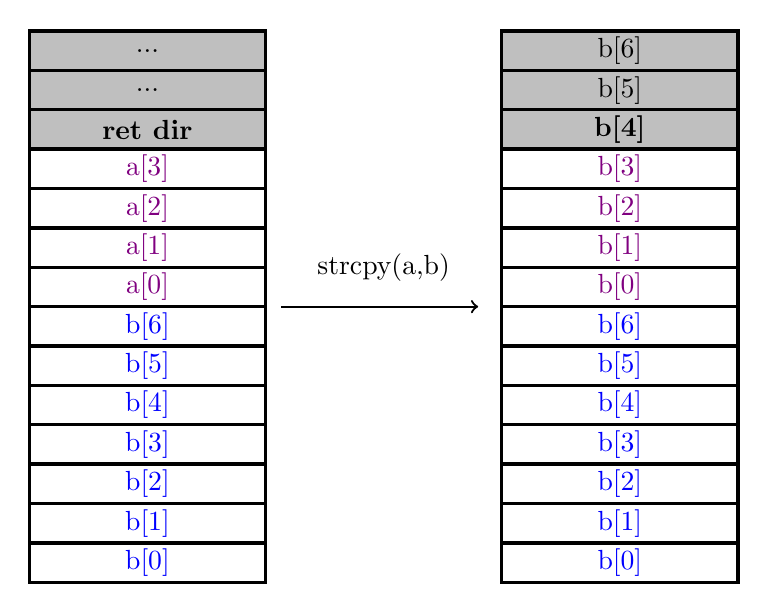
\begin{tikzpicture}
            %% stack
            \draw[black, very thick] (0,0)   rectangle (3,0.5);
            \draw[black, very thick] (0,0.5) rectangle (3,1);
            \draw[black, very thick] (0,1)   rectangle (3,1.5);
            \draw[black, very thick] (0,1.5) rectangle (3,2);
            \draw[black, very thick] (0,2)   rectangle (3,2.5);
            \draw[black, very thick] (0,2.5) rectangle (3,3);
            \draw[black, very thick] (0,3)   rectangle (3,3.5);
            \draw[black, very thick] (0,3.5) rectangle (3,4);
            \draw[black, very thick] (0,4)   rectangle (3,4.5);
            \draw[black, very thick] (0,4.5) rectangle (3,5);
            \draw[black, very thick] (0,5) rectangle (3,5.5);
            \draw[black, very thick, fill=lightgray] (0,5.5) rectangle (3,6);
            \draw[black, very thick, fill=lightgray] (0,6) rectangle (3,6.5);
            \draw[black, very thick, fill=lightgray] (0,6.5) rectangle (3,7);

            \node at (1.5,0.25) {\textcolor{blue}{b[0]}};
            \node at (1.5,0.75) {\textcolor{blue}{b[1]}};
            \node at (1.5,1.25) {\textcolor{blue}{b[2]}};
            \node at (1.5,1.75) {\textcolor{blue}{b[3]}};
            \node at (1.5,2.25) {\textcolor{blue}{b[4]}};
            \node at (1.5,2.75) {\textcolor{blue}{b[5]}};
            \node at (1.5,3.25) {\textcolor{blue}{b[6]}};
            \node at (1.5,3.75) {\textcolor{violet}{a[0]}};
            \node at (1.5,4.25) {\textcolor{violet}{a[1]}};
            \node at (1.5,4.75) {\textcolor{violet}{a[2]}};
            \node at (1.5,5.25) {\textcolor{violet}{a[3]}};
            \node at (1.5,5.75) {\textbf{ret dir}};
            \node at (1.5,6.25) {...};
            \node at (1.5,6.75) {...};


            %% stack
            \draw[black, very thick] (6,0)   rectangle (9,0.5);
            \draw[black, very thick] (6,0.5) rectangle (9,1);
            \draw[black, very thick] (6,1)   rectangle (9,1.5);
            \draw[black, very thick] (6,1.5) rectangle (9,2);
            \draw[black, very thick] (6,2)   rectangle (9,2.5);
            \draw[black, very thick] (6,2.5) rectangle (9,3);
            \draw[black, very thick] (6,3)   rectangle (9,3.5);
            \draw[black, very thick] (6,3.5) rectangle (9,4);
            \draw[black, very thick] (6,4)   rectangle (9,4.5);
            \draw[black, very thick] (6,4.5) rectangle (9,5);
            \draw[black, very thick] (6,5)   rectangle (9,5.5);
            \draw[black, very thick, fill=lightgray] (6,5.5) rectangle (9,6);
            \draw[black, very thick, fill=lightgray] (6,6) rectangle   (9,6.5);
            \draw[black, very thick, fill=lightgray] (6,6.5) rectangle (9,7);

            \node at (7.5,0.25) {\textcolor{blue}{b[0]}};
            \node at (7.5,0.75) {\textcolor{blue}{b[1]}};
            \node at (7.5,1.25) {\textcolor{blue}{b[2]}};
            \node at (7.5,1.75) {\textcolor{blue}{b[3]}};
            \node at (7.5,2.25) {\textcolor{blue}{b[4]}};
            \node at (7.5,2.75) {\textcolor{blue}{b[5]}};
            \node at (7.5,3.25) {\textcolor{blue}{b[6]}};
            \node at (7.5,3.75) {\textcolor{violet}{b[0]}};
            \node at (7.5,4.25) {\textcolor{violet}{b[1]}};
            \node at (7.5,4.75) {\textcolor{violet}{b[2]}};
            \node at (7.5,5.25) {\textcolor{violet}{b[3]}};
            \node at (7.5,5.75) {\textbf{b[4]}};
            \node at (7.5,6.25) {b[5]};
            \node at (7.5,6.75) {b[6]};

            \draw[->, thick] (3.2,3.5) -- (5.7,3.5);

            \node at (4.5,4) {strcpy(a,b)};

        \end{tikzpicture}
    \end{figure}
    
\end{frame}

\begin{frame}
    \frametitle{Contramedidas}
    \begin{itemize}
        \item Programación fuertemente tipada y validar longitudes.
        \item No utilizar funciones de biblioteca y diseñar de forma segura.
        \item Minimizar los puntos de error.
        \item Verificar los retornos.
        \item Colocar la pila como no ejecutable y agregar canarios.
    \end{itemize}
\end{frame}




\begin{frame}
    \frametitle{Programación orientada a los retornos\footnote{\textit{Return-Oriented Programing}}}
    Permite explotar errores de memoria sin inyectar código usando el código del mismo proceso.\\

    \vs
    
    Aprovechando la instrucción \return pues realizan un \textbf{salto} y \textbf{cambia el estado}.\\
    
\end{frame}

\begin{frame}
    \frametitle{Conjunto de \textit{gadgets}}
    \begin{block}{Definición}
        Uso de secuencia de instrucciones que {\only<2->{\color{blue}}ya están presentes en el proceso}, en particular tienen permisos de ejecución. El stack es usado como lugar para almacenar el ``código''.
    \end{block}

    Las secuencias deben terminar en la instrucción \return así permiten definir una máquina virtual.\vs
    
    \vs
    
    Se puede buscar posibles \textit{Gadget} de manera automatizada dendentro del código compilado.

\end{frame}

\begin{frame}
    \frametitle{Convención de llamada}
    \only<1>{
        \begin{figure}[h]
            \centering
            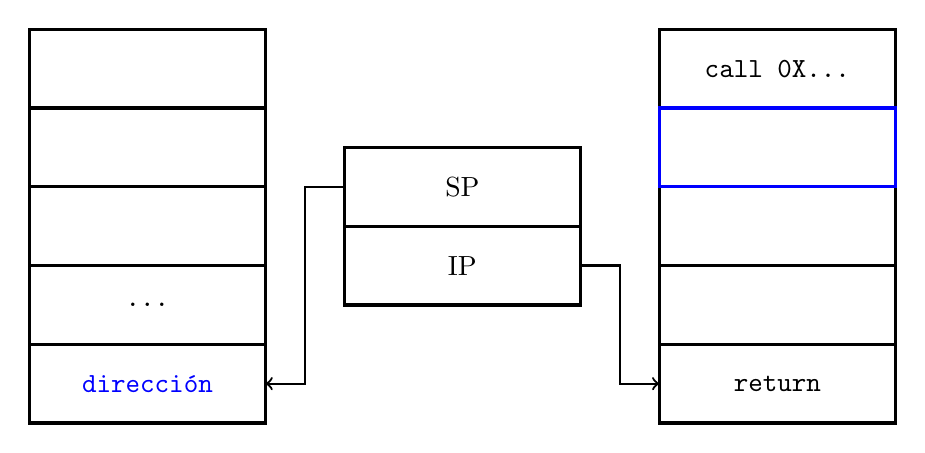
\begin{tikzpicture}
                %% stack
                \draw[black, very thick] (0,0) rectangle (3,1);
                \draw[black, very thick] (0,1) rectangle (3,2);
                \draw[black, very thick] (0,2) rectangle (3,3);
                \draw[black, very thick] (0,3) rectangle (3,4);
                \draw[black, very thick] (0,4) rectangle (3,5);

                \node at (1.5,1.5) {\texttt{...}};
                \node at (1.5,0.5) {\textcolor{blue}{\texttt{dirección}}};

                
                %SP
                \draw[black, very thick] (4,2.5) rectangle (7,3.5);
                \node at (5.5,3) {SP};
                \draw[->, thick] (4,3) -- (3.5,3) |- (3,0.5);

                %IP
                \draw[black, very thick] (4,1.5) rectangle (7,2.5);
                \node at (5.5,2) {IP};
                \draw[->, thick] (7,2) -- (7.5,2) |- (8,0.5);


                %% Código

                \draw[black, very thick] (8,0) rectangle (11,1);
                \draw[black, very thick] (8,1) rectangle (11,2);
                \draw[black, very thick] (8,2) rectangle (11,3);
                \draw[black, very thick] (8,4) rectangle (11,5);
                \draw[blue , very thick] (8,3) rectangle (11,4);

                \node at (9.5,0.5) {\return};
                \node at (9.5,4.5) {\texttt{call 0X...}};


            \end{tikzpicture}
            \caption{Estado de los registro para la pila e instrucciones antes de un \return.}
        \end{figure}

    }
    \pause
    \only<2>{
        \begin{figure}[h]
            \centering
            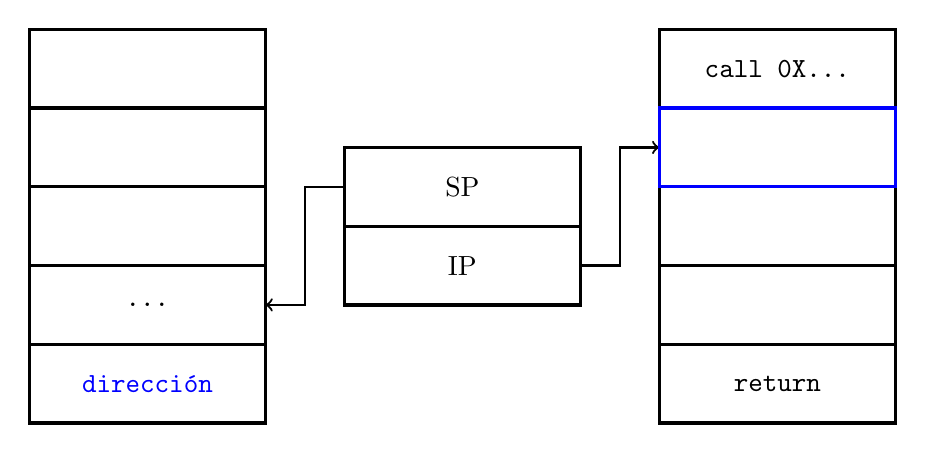
\begin{tikzpicture}
                %% stack
                \draw[black, very thick] (0,0) rectangle (3,1);
                \draw[black, very thick] (0,1) rectangle (3,2);
                \draw[black, very thick] (0,2) rectangle (3,3);
                \draw[black, very thick] (0,3) rectangle (3,4);
                \draw[black, very thick] (0,4) rectangle (3,5);

                \node at (1.5,1.5) {\texttt{...}};
                \node at (1.5,0.5) {\textcolor{blue}{\texttt{dirección}}};

                
                %SP
                \draw[black, very thick] (4,2.5) rectangle (7,3.5);
                \node at (5.5,3) {SP};
                \draw[->, thick] (4,3) -- (3.5,3) |- (3,1.5);

                %IP
                \draw[black, very thick] (4,1.5) rectangle (7,2.5);
                \node at (5.5,2) {IP};
                \draw[->, thick] (7,2) -- (7.5,2) |- (8,3.5);


                %% Código

                \draw[black, very thick] (8,0) rectangle (11,1);
                \draw[black, very thick] (8,1) rectangle (11,2);
                \draw[black, very thick] (8,2) rectangle (11,3);
                \draw[black, very thick] (8,4) rectangle (11,5);
                \draw[blue , very thick] (8,3) rectangle (11,4);

                \node at (9.5,0.5) {\return};
                \node at (9.5,4.5) {\texttt{call 0X...}};


            \end{tikzpicture}
            \caption{Estado de los registro para la pila e instrucciones después de un \return.}
        \end{figure}
    }
\end{frame}

\begin{frame}
    \frametitle{Contramedidas}
    \begin{itemize}
        \item Comparar la cantidad de \texttt{call} y \texttt{ret}. 
        \item Validar el invariante de \textit{last-in}, \textit{first-out}.
        \item No usar la instrucción \return.
    \end{itemize}
\end{frame}

\begin{frame}
    \frametitle{Programación orientada a los retornos sin retornos\footnote{\textit{Return-Oriented Programing without Returns}}}
    Se asume:

    \begin{itemize}
        \item Modelo de lectura o ejecución exclusivos ($W \oplus X$).
        \item Contramedidas para la programación orientada a los retornos.
    \end{itemize}
    \vs
    Necesitamos otros conjunto de instrucciones con las propiedades del \return:
    \begin{enumerate}
        \item Trasferir el control de ejecución.
        \item Actualizar el estado del proceso.
    \end{enumerate}
\end{frame}

\begin{frame}
    \frametitle{Si no usamos \return}
    \only<1>{
        \begin{figure}[h]
            \centering
            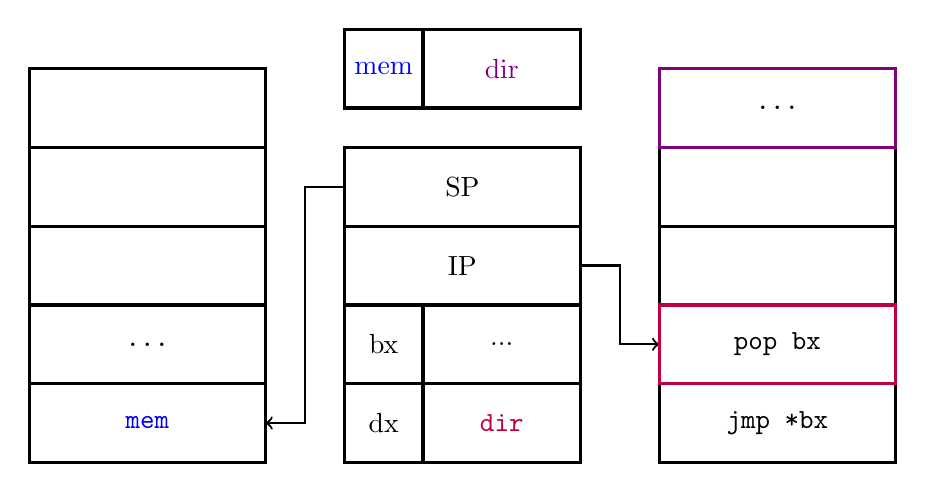
\begin{tikzpicture}
                %% stack
                \draw[black, very thick] (0,0) rectangle (3,1);
                \draw[black, very thick] (0,1) rectangle (3,2);
                \draw[black, very thick] (0,2) rectangle (3,3);
                \draw[black, very thick] (0,3) rectangle (3,4);
                \draw[black, very thick] (0,4) rectangle (3,5);

                \node at (1.5,1.5) {\texttt{...}};
                \node at (1.5,0.5) {\textcolor{blue}{\texttt{mem}}};

                
                %SP
                \draw[black, very thick] (4,3) rectangle (7,4);
                \node at (5.5,3.5) {SP};
                \draw[->, thick] (4,3.5) -- (3.5,3.5) |- (3,0.5);

                %IP
                \draw[black, very thick] (4,2) rectangle (7,3);
                \node at (5.5,2.5) {IP};
                \draw[->, thick] (7,2.5) -- (7.5,2.5) |- (8,1.5);

                %BX
                \draw[black, very thick] (4,1) rectangle (5,2);
                \draw[black, very thick] (5,1) rectangle (7,2);
                \node at (4.5,1.5) {bx};
                \node at (6,1.5)   {...};

                %DX
                \draw[black, very thick] (4,0) rectangle (5,1);
                \draw[black, very thick] (5,0) rectangle (7,1);
                \node at (4.5,0.5) {dx};
                \node at (6,0.5)   {\textcolor{purple}{\texttt{dir}}};

                %MEM
                \draw[black, very thick] (4,4.5) rectangle (5,5.5);
                \draw[black, very thick] (5,4.5) rectangle (7,5.5);
                \node at (4.5,5) {\textcolor{blue}{mem}};
                \node at (6,5) {\textcolor{violet}{dir}};

                
                %% Código

                \draw[black, very thick] (8,0) rectangle (11,1);
                \draw[black, very thick] (8,2) rectangle (11,3);
                \draw[black, very thick] (8,3) rectangle (11,4);
                \draw[violet , very thick] (8,4) rectangle (11,5);
                \draw[purple, very thick] (8,1) rectangle (11,2);
                
                \node at (9.5,1.5) {\texttt{pop bx}};
                \node at (9.5,0.5) {\texttt{jmp *bx}};
                \node at (9.5,4.5) {\texttt{...}};

            \end{tikzpicture}
            \caption{Ejecución del ``trampolín'': \texttt{pop} saca de la pila y coloca en \textbf{bx}}
        \end{figure}

    }
    \pause
    \only<2>{
        \begin{figure}[h]
            \centering
            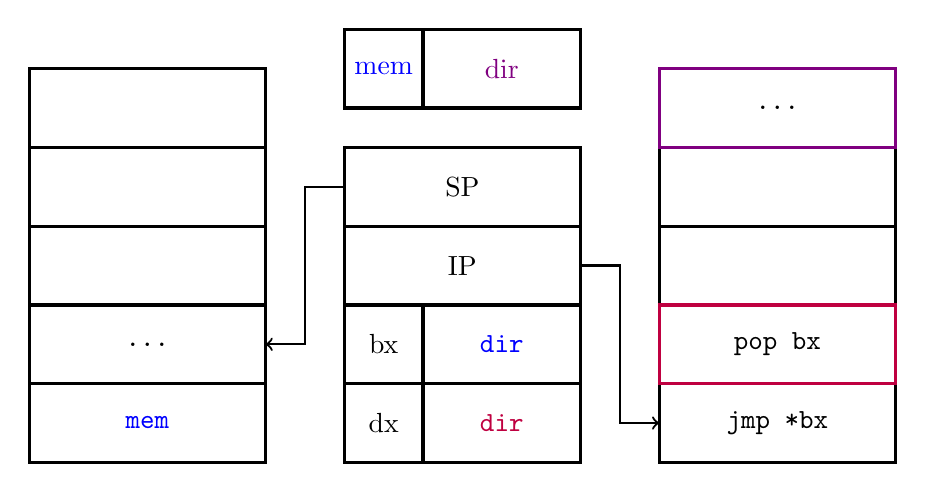
\begin{tikzpicture}
                %% stack
                \draw[black, very thick] (0,0) rectangle (3,1);
                \draw[black, very thick] (0,1) rectangle (3,2);
                \draw[black, very thick] (0,2) rectangle (3,3);
                \draw[black, very thick] (0,3) rectangle (3,4);
                \draw[black, very thick] (0,4) rectangle (3,5);

                \node at (1.5,1.5) {\texttt{...}};
                \node at (1.5,0.5) {\textcolor{blue}{\texttt{mem}}};

                
                %SP
                \draw[black, very thick] (4,3) rectangle (7,4);
                \node at (5.5,3.5) {SP};
                \draw[->, thick] (4,3.5) -- (3.5,3.5) |- (3,1.5);

                %IP
                \draw[black, very thick] (4,2) rectangle (7,3);
                \node at (5.5,2.5) {IP};
                \draw[->, thick] (7,2.5) -- (7.5,2.5) |- (8,0.5);

                %BX
                \draw[black, very thick] (4,1) rectangle (5,2);
                \draw[black, very thick] (5,1) rectangle (7,2);
                \node at (4.5,1.5) {bx};
                \node at (6,1.5)   {\textcolor{blue}{\texttt{dir}}};

                %DX
                \draw[black, very thick] (4,0) rectangle (5,1);
                \draw[black, very thick] (5,0) rectangle (7,1);
                \node at (4.5,0.5) {dx};
                \node at (6,0.5)   {\textcolor{purple}{\texttt{dir}}};

                %MEM
                \draw[black, very thick] (4,4.5) rectangle (5,5.5);
                \draw[black, very thick] (5,4.5) rectangle (7,5.5);
                \node at (4.5,5) {\textcolor{blue}{mem}};
                \node at (6,5) {\textcolor{violet}{dir}};
                
                %% Código

                \draw[black, very thick] (8,0) rectangle (11,1);
                \draw[black, very thick] (8,2) rectangle (11,3);
                \draw[black, very thick] (8,3) rectangle (11,4);
                \draw[violet , very thick] (8,4) rectangle (11,5);
                \draw[purple, very thick] (8,1) rectangle (11,2);
                
                \node at (9.5,1.5) {\texttt{pop bx}};
                \node at (9.5,0.5) {\texttt{jmp *bx}};
                \node at (9.5,4.5) {\texttt{...}};

            \end{tikzpicture}
            \caption{Ejecución del ``trampolín'': \texttt{jmp} salta a la dirección de \textbf{bx}}
        \end{figure}

    }
    \pause
    \only<3>{
        \begin{figure}[h]
            \centering
            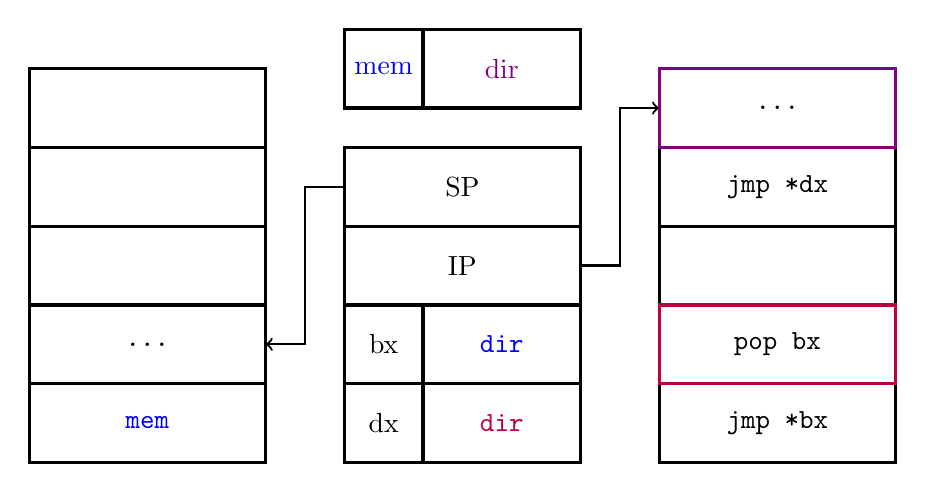
\begin{tikzpicture}
                %% stack
                \draw[black, very thick] (0,0) rectangle (3,1);
                \draw[black, very thick] (0,1) rectangle (3,2);
                \draw[black, very thick] (0,2) rectangle (3,3);
                \draw[black, very thick] (0,3) rectangle (3,4);
                \draw[black, very thick] (0,4) rectangle (3,5);

                \node at (1.5,1.5) {\texttt{...}};
                \node at (1.5,0.5) {\textcolor{blue}{\texttt{mem}}};

                
                %SP
                \draw[black, very thick] (4,3) rectangle (7,4);
                \node at (5.5,3.5) {SP};
                \draw[->, thick] (4,3.5) -- (3.5,3.5) |- (3,1.5);

                %IP
                \draw[black, very thick] (4,2) rectangle (7,3);
                \node at (5.5,2.5) {IP};
                \draw[->, thick] (7,2.5) -- (7.5,2.5) |- (8,4.5);

                %BX
                \draw[black, very thick] (4,1) rectangle (5,2);
                \draw[black, very thick] (5,1) rectangle (7,2);
                \node at (4.5,1.5) {bx};
                \node at (6,1.5)   {\textcolor{blue}{\texttt{dir}}};

                %DX
                \draw[black, very thick] (4,0) rectangle (5,1);
                \draw[black, very thick] (5,0) rectangle (7,1);
                \node at (4.5,0.5) {dx};
                \node at (6,0.5)   {\textcolor{purple}{\texttt{dir}}};

                %MEM
                \draw[black, very thick] (4,4.5) rectangle (5,5.5);
                \draw[black, very thick] (5,4.5) rectangle (7,5.5);
                \node at (4.5,5) {\textcolor{blue}{mem}};
                \node at (6,5) {\textcolor{violet}{dir}};

                
                %% Código

                \draw[black, very thick] (8,0) rectangle (11,1);
                \draw[black, very thick] (8,2) rectangle (11,3);
                \draw[black, very thick] (8,3) rectangle (11,4);
                \draw[violet , very thick] (8,4) rectangle (11,5);
                \draw[purple, very thick] (8,1) rectangle (11,2);
                
                \node at (9.5,1.5) {\texttt{pop bx}};
                \node at (9.5,0.5) {\texttt{jmp *bx}};
                \node at (9.5,4.5) {\texttt{...}};
                \node at (9.5,3.5) {\texttt{jmp *dx}};

            \end{tikzpicture}
            \caption{Ejecución del código del \textit{gadget}. Debe terminar con un salto al trampolín.}
        \end{figure}

    }
\end{frame}

\begin{frame}
    \frametitle{INTEL x86}
    En este caso el conjunto de \textit{gadgets} proviene de \texttt{libc} y \texttt{libul}. \\

    Los \textit{gadgets} son 19: \texttt{load} (\texttt{immediate}), \texttt{move}, \texttt{store}, \texttt{add} (\texttt{immediate}), \texttt{subtract}, \texttt{negate}, \texttt{and} (\texttt{immediate}), \texttt{or} (\texttt{immediate}), \texttt{xor} (\texttt{immediate}), \textit{complement}, \texttt{branch unconditional}, \texttt{branch conditional}, \texttt{set less than} y \texttt{call}. 
\end{frame}

\begin{frame}
    \frametitle{INTEL x86: Observaciones}
    \begin{itemize}
        % \item 
        \item Se busca que las operaciones actualicen valores en memoria.
        % \item Las interacciones con memoria requieren registros intermedios, porque se usan 2 niveles de indirección.
        \item Las ramas condicionales actualizan valores de memoria y no el registro de instrucciones.
        \item La convención para hacer llamadas a funciones utilizada en el paper no es la actual en Linux.
    \end{itemize}
\end{frame}

\begin{frame}
    \frametitle{INTEL x86: \textit{gadget} ($\le$)}
    \begin{figure}
        \centering
        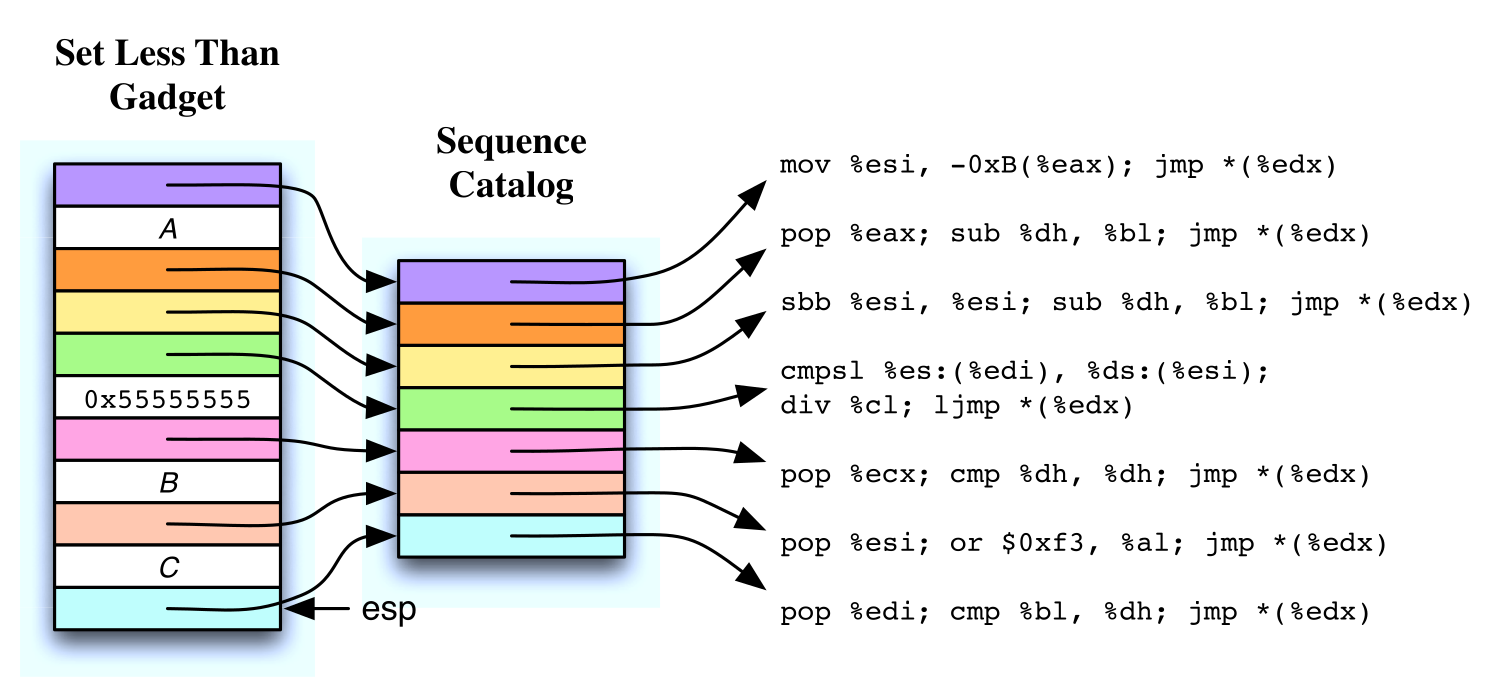
\includegraphics[scale=0.2]{gadgetx86.png}
    \end{figure}
\end{frame}

\begin{frame}
    \frametitle{ARM}

   En ARM no hay una convención de llamada mediante instrucciones.

    \vs

    Hay menos registros pero todos son de propósito general y pueden ser modificados.

    \vs

    No hay instrucciones \texttt{call} y \texttt{ret}. En su lugar se tienen \texttt{bl} y \texttt{blx}.

\end{frame}

\begin{frame}
    \frametitle{ARM}
    \only<1>{
        \begin{figure}[h]
        \centering
        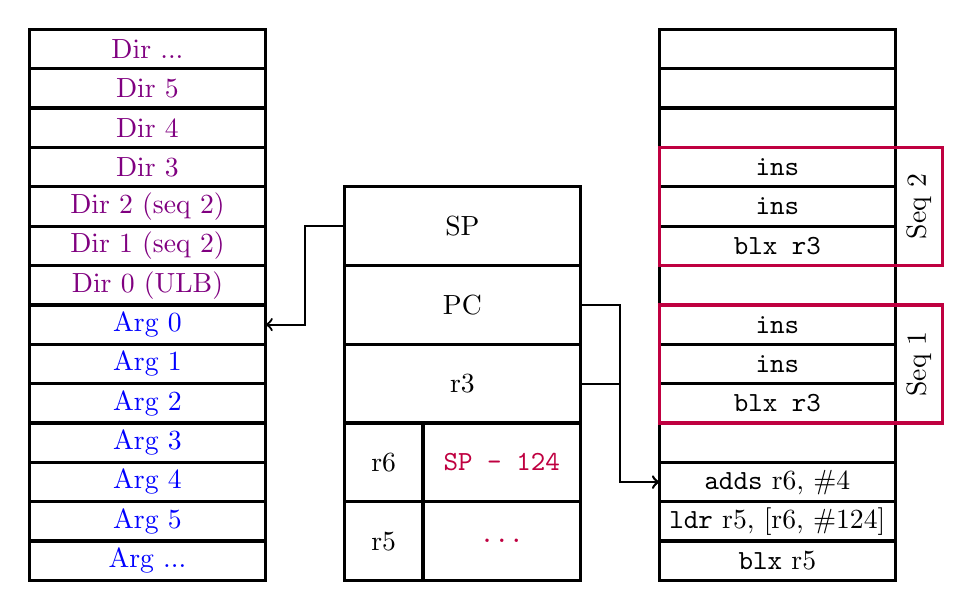
\begin{tikzpicture}
            %% stack
            \draw[black, very thick] (0,0)   rectangle (3,0.5);
            \draw[black, very thick] (0,0.5) rectangle (3,1);
            \draw[black, very thick] (0,1)   rectangle (3,1.5);
            \draw[black, very thick] (0,1.5) rectangle (3,2);
            \draw[black, very thick] (0,2)   rectangle (3,2.5);
            \draw[black, very thick] (0,2.5) rectangle (3,3);
            \draw[black, very thick] (0,3)   rectangle (3,3.5);
            \draw[black, very thick] (0,3.5) rectangle (3,4);
            \draw[black, very thick] (0,4)   rectangle (3,4.5);
            \draw[black, very thick] (0,4.5) rectangle (3,5);
            \draw[black, very thick] (0,5)   rectangle (3,5.5);
            \draw[black, very thick] (0,5.5) rectangle (3,6);
            \draw[black, very thick] (0,6)   rectangle (3,6.5);
            \draw[black, very thick] (0,6.5) rectangle (3,7);

            \node at (1.5,0.25) {\textcolor{blue}{Arg ...}};
            \node at (1.5,0.75) {\textcolor{blue}{Arg 5}};
            \node at (1.5,1.25) {\textcolor{blue}{Arg 4}};
            \node at (1.5,1.75) {\textcolor{blue}{Arg 3}};
            \node at (1.5,2.25) {\textcolor{blue}{Arg 2}};
            \node at (1.5,2.75) {\textcolor{blue}{Arg 1}};
            \node at (1.5,3.25) {\textcolor{blue}{Arg 0}};
            \node at (1.5,3.75) {\textcolor{violet}{Dir 0 (ULB)}};
            \node at (1.5,4.25) {\textcolor{violet}{Dir 1 (seq 2)}};
            \node at (1.5,4.75) {\textcolor{violet}{Dir 2 (seq 2)}};
            \node at (1.5,5.25) {\textcolor{violet}{Dir 3}};
            \node at (1.5,5.75) {\textcolor{violet}{Dir 4}};
            \node at (1.5,6.25) {\textcolor{violet}{Dir 5}};
            \node at (1.5,6.75) {\textcolor{violet}{Dir ...}};


            %% Code
            \draw[black, very thick] (8,0)   rectangle (11,0.5);
            \draw[black, very thick] (8,0.5) rectangle (11,1);
            \draw[black, very thick] (8,1)   rectangle (11,1.5);
            \draw[black, very thick] (8,1.5) rectangle (11,2);
            \draw[black, very thick] (8,2)   rectangle (11,2.5);
            \draw[black, very thick] (8,2.5) rectangle (11,3);
            \draw[black, very thick] (8,3)   rectangle (11,3.5);
            \draw[black, very thick] (8,3.5) rectangle (11,4);
            \draw[black, very thick] (8,4)   rectangle (11,4.5);
            \draw[black, very thick] (8,4.5) rectangle (11,5);
            \draw[black, very thick] (8,5)   rectangle (11,5.5);
            \draw[black, very thick] (8,5.5) rectangle (11,6);
            \draw[black, very thick] (8,6) rectangle   (11,6.5);
            \draw[black, very thick] (8,6.5) rectangle (11,7);

            \node at (9.5,0.25) {\texttt{blx} r5};
            \node at (9.5,0.75) {\texttt{ldr} r5, [r6, \#124]};
            \node at (9.5,1.25) {\texttt{adds} r6, \#4};
            \node at (9.5,1.75) {};
            \node at (9.5,2.25) {\texttt{blx r3}};
            \node at (9.5,2.75) {\texttt{ins}};
            \node at (9.5,3.25) {\texttt{ins}};
            \node at (9.5,3.75) {};
            \node at (9.5,4.25) {\texttt{blx r3}};
            \node at (9.5,4.75) {\texttt{ins}};
            \node at (9.5,5.25) {\texttt{ins}};
            \node at (9.5,5.75) {};
            \node at (9.5,6.25) {};
            \node at (9.5,6.75) {};

            % Seq 1
            \node[rotate=90] at (11.3,2.75) {Seq 1};
            \draw[purple, very thick] (8,2) rectangle (11.6,3.5);

            % Seq 2
            \node[rotate=90] at (11.3,4.75) {Seq 2};
            \draw[purple, very thick] (8,4) rectangle (11.6,5.5);


            %SP
            \draw[black, very thick] (4,4) rectangle (7,5);
            \node at (5.5,4.5) {SP};
            \draw[->, thick] (4,4.5) -- (3.5,4.5) |- (3,3.25);

            %PC
            \draw[black, very thick] (4,3) rectangle (7,4);
            \node at (5.5,3.5) {PC};
            \draw[->, thick] (7,3.5) -- (7.5,3.5) |- (8,1.25);

            %R3
            \draw[black, very thick] (4,2) rectangle (7,3);
            \node at (5.5,2.5) {r3};
            \draw[->, thick] (7,2.5) -- (7.5,2.5) |- (8,1.25);

            %R6
            \draw[black, very thick] (4,1) rectangle (7,2);
            \draw[black, very thick] (5,1) rectangle (7,2);
            \node at (4.5,1.5) {r6};
            \node at (6,1.5)   {\textcolor{purple}{\texttt{SP - 124}}};

            %R5
            \draw[black, very thick] (4,0) rectangle (5,1);
            \draw[black, very thick] (5,0) rectangle (7,1);
            \node at (4.5,0.5) {r5};
            \node at (6,0.5)   {\textcolor{purple}{\texttt{...}}};

        \end{tikzpicture}
        \end{figure}

    }
    \pause
    \only<2>{

        \begin{figure}[h]
            \centering
            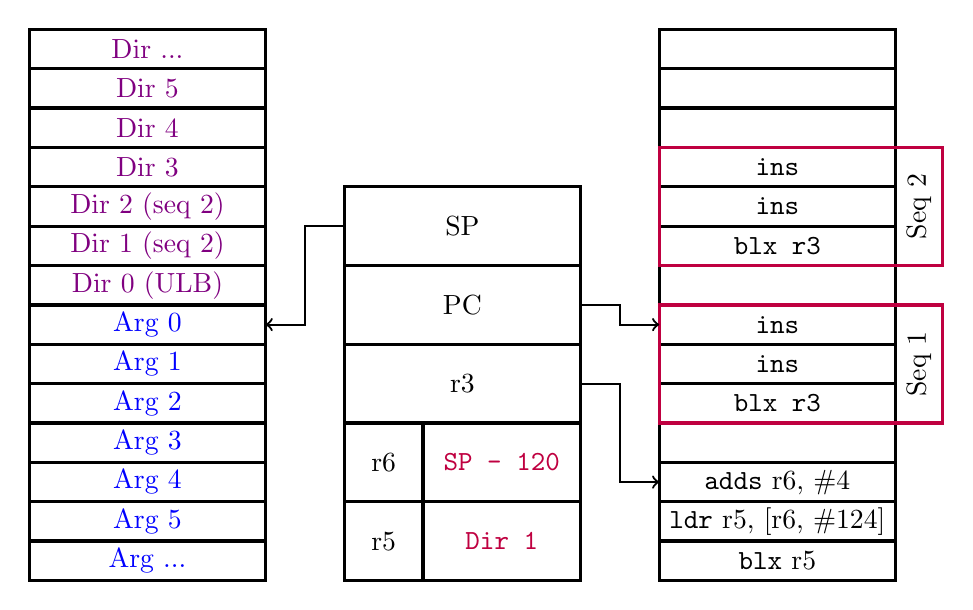
\begin{tikzpicture}
                %% stack
                \draw[black, very thick] (0,0)   rectangle (3,0.5);
                \draw[black, very thick] (0,0.5) rectangle (3,1);
                \draw[black, very thick] (0,1)   rectangle (3,1.5);
                \draw[black, very thick] (0,1.5) rectangle (3,2);
                \draw[black, very thick] (0,2)   rectangle (3,2.5);
                \draw[black, very thick] (0,2.5) rectangle (3,3);
                \draw[black, very thick] (0,3)   rectangle (3,3.5);
                \draw[black, very thick] (0,3.5) rectangle (3,4);
                \draw[black, very thick] (0,4)   rectangle (3,4.5);
                \draw[black, very thick] (0,4.5) rectangle (3,5);
                \draw[black, very thick] (0,5)   rectangle (3,5.5);
                \draw[black, very thick] (0,5.5) rectangle (3,6);
                \draw[black, very thick] (0,6)   rectangle (3,6.5);
                \draw[black, very thick] (0,6.5) rectangle (3,7);
    
                \node at (1.5,0.25) {\textcolor{blue}{Arg ...}};
                \node at (1.5,0.75) {\textcolor{blue}{Arg 5}};
                \node at (1.5,1.25) {\textcolor{blue}{Arg 4}};
                \node at (1.5,1.75) {\textcolor{blue}{Arg 3}};
                \node at (1.5,2.25) {\textcolor{blue}{Arg 2}};
                \node at (1.5,2.75) {\textcolor{blue}{Arg 1}};
                \node at (1.5,3.25) {\textcolor{blue}{Arg 0}};
                \node at (1.5,3.75) {\textcolor{violet}{Dir 0 (ULB)}};
                \node at (1.5,4.25) {\textcolor{violet}{Dir 1 (seq 2)}};
                \node at (1.5,4.75) {\textcolor{violet}{Dir 2 (seq 2)}};
                \node at (1.5,5.25) {\textcolor{violet}{Dir 3}};
                \node at (1.5,5.75) {\textcolor{violet}{Dir 4}};
                \node at (1.5,6.25) {\textcolor{violet}{Dir 5}};
                \node at (1.5,6.75) {\textcolor{violet}{Dir ...}};
    
    
                %% Code
                \draw[black, very thick] (8,0)   rectangle (11,0.5);
                \draw[black, very thick] (8,0.5) rectangle (11,1);
                \draw[black, very thick] (8,1)   rectangle (11,1.5);
                \draw[black, very thick] (8,1.5) rectangle (11,2);
                \draw[black, very thick] (8,2)   rectangle (11,2.5);
                \draw[black, very thick] (8,2.5) rectangle (11,3);
                \draw[black, very thick] (8,3)   rectangle (11,3.5);
                \draw[black, very thick] (8,3.5) rectangle (11,4);
                \draw[black, very thick] (8,4)   rectangle (11,4.5);
                \draw[black, very thick] (8,4.5) rectangle (11,5);
                \draw[black, very thick] (8,5)   rectangle (11,5.5);
                \draw[black, very thick] (8,5.5) rectangle (11,6);
                \draw[black, very thick] (8,6) rectangle   (11,6.5);
                \draw[black, very thick] (8,6.5) rectangle (11,7);
    
                \node at (9.5,0.25) {\texttt{blx} r5};
                \node at (9.5,0.75) {\texttt{ldr} r5, [r6, \#124]};
                \node at (9.5,1.25) {\texttt{adds} r6, \#4};
                \node at (9.5,1.75) {};
                \node at (9.5,2.25) {\texttt{blx r3}};
                \node at (9.5,2.75) {\texttt{ins}};
                \node at (9.5,3.25) {\texttt{ins}};
                \node at (9.5,3.75) {};
                \node at (9.5,4.25) {\texttt{blx r3}};
                \node at (9.5,4.75) {\texttt{ins}};
                \node at (9.5,5.25) {\texttt{ins}};
                \node at (9.5,5.75) {};
                \node at (9.5,6.25) {};
                \node at (9.5,6.75) {};
    
                % Seq 1
                \node[rotate=90] at (11.3,2.75) {Seq 1};
                \draw[purple, very thick] (8,2) rectangle (11.6,3.5);
    
                % Seq 2
                \node[rotate=90] at (11.3,4.75) {Seq 2};
                \draw[purple, very thick] (8,4) rectangle (11.6,5.5);
    
    
                %SP
                \draw[black, very thick] (4,4) rectangle (7,5);
                \node at (5.5,4.5) {SP};
                \draw[->, thick] (4,4.5) -- (3.5,4.5) |- (3,3.25);
    
                %PC
                \draw[black, very thick] (4,3) rectangle (7,4);
                \node at (5.5,3.5) {PC};
                \draw[->, thick] (7,3.5) -- (7.5,3.5) |- (8,3.25);
    
                %R3
                \draw[black, very thick] (4,2) rectangle (7,3);
                \node at (5.5,2.5) {r3};
                \draw[->, thick] (7,2.5) -- (7.5,2.5) |- (8,1.25);
    
                %R6
                \draw[black, very thick] (4,1) rectangle (7,2);
                \draw[black, very thick] (5,1) rectangle (7,2);
                \node at (4.5,1.5) {r6};
                \node at (6,1.5)   {\textcolor{purple}{\texttt{SP - 120}}};
    
                %R5
                \draw[black, very thick] (4,0) rectangle (5,1);
                \draw[black, very thick] (5,0) rectangle (7,1);
                \node at (4.5,0.5) {r5};
                \node at (6,0.5)   {\textcolor{purple}{\texttt{Dir 1}}};
    
            \end{tikzpicture}
        \end{figure}
    }
    \pause
    \only<3>{

        \begin{figure}[h]
            \centering
            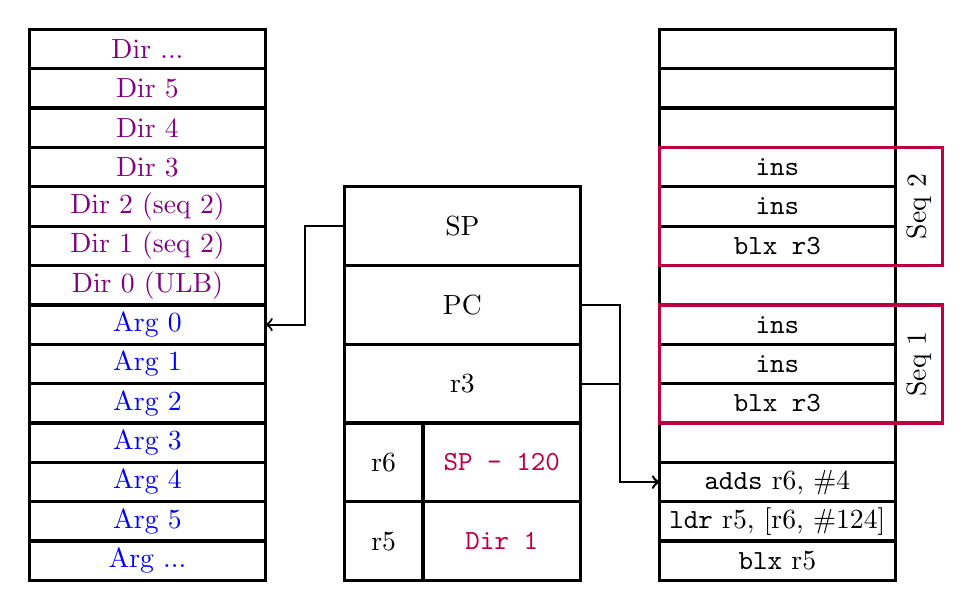
\begin{tikzpicture}
                %% stack
                \draw[black, very thick] (0,0)   rectangle (3,0.5);
                \draw[black, very thick] (0,0.5) rectangle (3,1);
                \draw[black, very thick] (0,1)   rectangle (3,1.5);
                \draw[black, very thick] (0,1.5) rectangle (3,2);
                \draw[black, very thick] (0,2)   rectangle (3,2.5);
                \draw[black, very thick] (0,2.5) rectangle (3,3);
                \draw[black, very thick] (0,3)   rectangle (3,3.5);
                \draw[black, very thick] (0,3.5) rectangle (3,4);
                \draw[black, very thick] (0,4)   rectangle (3,4.5);
                \draw[black, very thick] (0,4.5) rectangle (3,5);
                \draw[black, very thick] (0,5)   rectangle (3,5.5);
                \draw[black, very thick] (0,5.5) rectangle (3,6);
                \draw[black, very thick] (0,6)   rectangle (3,6.5);
                \draw[black, very thick] (0,6.5) rectangle (3,7);
    
                \node at (1.5,0.25) {\textcolor{blue}{Arg ...}};
                \node at (1.5,0.75) {\textcolor{blue}{Arg 5}};
                \node at (1.5,1.25) {\textcolor{blue}{Arg 4}};
                \node at (1.5,1.75) {\textcolor{blue}{Arg 3}};
                \node at (1.5,2.25) {\textcolor{blue}{Arg 2}};
                \node at (1.5,2.75) {\textcolor{blue}{Arg 1}};
                \node at (1.5,3.25) {\textcolor{blue}{Arg 0}};
                \node at (1.5,3.75) {\textcolor{violet}{Dir 0 (ULB)}};
                \node at (1.5,4.25) {\textcolor{violet}{Dir 1 (seq 2)}};
                \node at (1.5,4.75) {\textcolor{violet}{Dir 2 (seq 2)}};
                \node at (1.5,5.25) {\textcolor{violet}{Dir 3}};
                \node at (1.5,5.75) {\textcolor{violet}{Dir 4}};
                \node at (1.5,6.25) {\textcolor{violet}{Dir 5}};
                \node at (1.5,6.75) {\textcolor{violet}{Dir ...}};
    
    
                %% Code
                \draw[black, very thick] (8,0)   rectangle (11,0.5);
                \draw[black, very thick] (8,0.5) rectangle (11,1);
                \draw[black, very thick] (8,1)   rectangle (11,1.5);
                \draw[black, very thick] (8,1.5) rectangle (11,2);
                \draw[black, very thick] (8,2)   rectangle (11,2.5);
                \draw[black, very thick] (8,2.5) rectangle (11,3);
                \draw[black, very thick] (8,3)   rectangle (11,3.5);
                \draw[black, very thick] (8,3.5) rectangle (11,4);
                \draw[black, very thick] (8,4)   rectangle (11,4.5);
                \draw[black, very thick] (8,4.5) rectangle (11,5);
                \draw[black, very thick] (8,5)   rectangle (11,5.5);
                \draw[black, very thick] (8,5.5) rectangle (11,6);
                \draw[black, very thick] (8,6) rectangle   (11,6.5);
                \draw[black, very thick] (8,6.5) rectangle (11,7);
    
                \node at (9.5,0.25) {\texttt{blx} r5};
                \node at (9.5,0.75) {\texttt{ldr} r5, [r6, \#124]};
                \node at (9.5,1.25) {\texttt{adds} r6, \#4};
                \node at (9.5,1.75) {};
                \node at (9.5,2.25) {\texttt{blx r3}};
                \node at (9.5,2.75) {\texttt{ins}};
                \node at (9.5,3.25) {\texttt{ins}};
                \node at (9.5,3.75) {};
                \node at (9.5,4.25) {\texttt{blx r3}};
                \node at (9.5,4.75) {\texttt{ins}};
                \node at (9.5,5.25) {\texttt{ins}};
                \node at (9.5,5.75) {};
                \node at (9.5,6.25) {};
                \node at (9.5,6.75) {};
    
                % Seq 1
                \node[rotate=90] at (11.3,2.75) {Seq 1};
                \draw[purple, very thick] (8,2) rectangle (11.6,3.5);
    
                % Seq 2
                \node[rotate=90] at (11.3,4.75) {Seq 2};
                \draw[purple, very thick] (8,4) rectangle (11.6,5.5);
    
    
                %SP
                \draw[black, very thick] (4,4) rectangle (7,5);
                \node at (5.5,4.5) {SP};
                \draw[->, thick] (4,4.5) -- (3.5,4.5) |- (3,3.25);
    
                %PC
                \draw[black, very thick] (4,3) rectangle (7,4);
                \node at (5.5,3.5) {PC};
                \draw[->, thick] (7,3.5) -- (7.5,3.5) |- (8,1.25);
    
                %R3
                \draw[black, very thick] (4,2) rectangle (7,3);
                \node at (5.5,2.5) {r3};
                \draw[->, thick] (7,2.5) -- (7.5,2.5) |- (8,1.25);
    
                %R6
                \draw[black, very thick] (4,1) rectangle (7,2);
                \draw[black, very thick] (5,1) rectangle (7,2);
                \node at (4.5,1.5) {r6};
                \node at (6,1.5)   {\textcolor{purple}{\texttt{SP - 120}}};
    
                %R5
                \draw[black, very thick] (4,0) rectangle (5,1);
                \draw[black, very thick] (5,0) rectangle (7,1);
                \node at (4.5,0.5) {r5};
                \node at (6,0.5)   {\textcolor{purple}{\texttt{Dir 1}}};
    
            \end{tikzpicture}
        \end{figure}

    }
    \pause
    \only<4>{

        \begin{figure}[h]
            \centering
            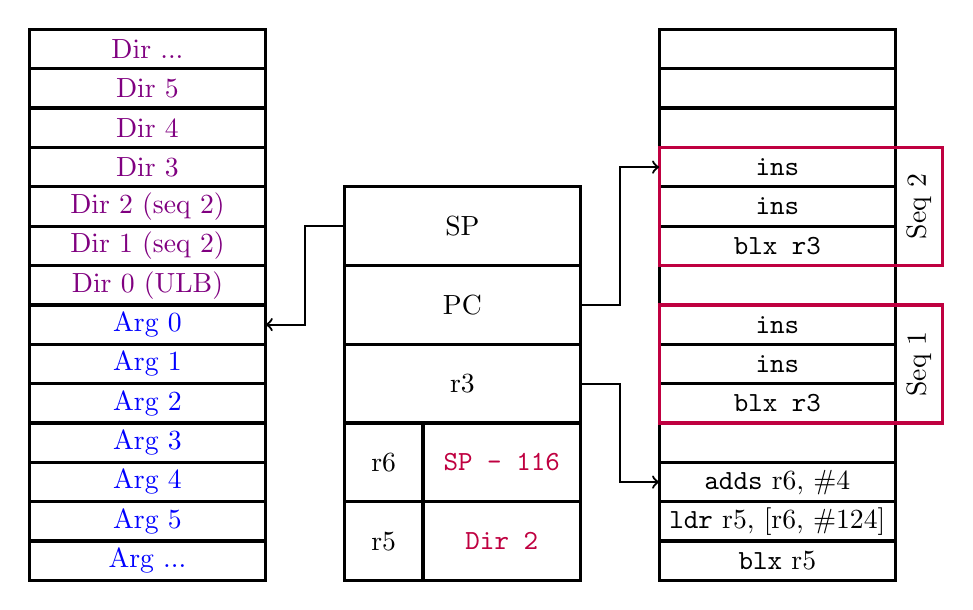
\begin{tikzpicture}
                %% stack
                \draw[black, very thick] (0,0)   rectangle (3,0.5);
                \draw[black, very thick] (0,0.5) rectangle (3,1);
                \draw[black, very thick] (0,1)   rectangle (3,1.5);
                \draw[black, very thick] (0,1.5) rectangle (3,2);
                \draw[black, very thick] (0,2)   rectangle (3,2.5);
                \draw[black, very thick] (0,2.5) rectangle (3,3);
                \draw[black, very thick] (0,3)   rectangle (3,3.5);
                \draw[black, very thick] (0,3.5) rectangle (3,4);
                \draw[black, very thick] (0,4)   rectangle (3,4.5);
                \draw[black, very thick] (0,4.5) rectangle (3,5);
                \draw[black, very thick] (0,5)   rectangle (3,5.5);
                \draw[black, very thick] (0,5.5) rectangle (3,6);
                \draw[black, very thick] (0,6)   rectangle (3,6.5);
                \draw[black, very thick] (0,6.5) rectangle (3,7);
    
                \node at (1.5,0.25) {\textcolor{blue}{Arg ...}};
                \node at (1.5,0.75) {\textcolor{blue}{Arg 5}};
                \node at (1.5,1.25) {\textcolor{blue}{Arg 4}};
                \node at (1.5,1.75) {\textcolor{blue}{Arg 3}};
                \node at (1.5,2.25) {\textcolor{blue}{Arg 2}};
                \node at (1.5,2.75) {\textcolor{blue}{Arg 1}};
                \node at (1.5,3.25) {\textcolor{blue}{Arg 0}};
                \node at (1.5,3.75) {\textcolor{violet}{Dir 0 (ULB)}};
                \node at (1.5,4.25) {\textcolor{violet}{Dir 1 (seq 2)}};
                \node at (1.5,4.75) {\textcolor{violet}{Dir 2 (seq 2)}};
                \node at (1.5,5.25) {\textcolor{violet}{Dir 3}};
                \node at (1.5,5.75) {\textcolor{violet}{Dir 4}};
                \node at (1.5,6.25) {\textcolor{violet}{Dir 5}};
                \node at (1.5,6.75) {\textcolor{violet}{Dir ...}};
    
    
                %% Code
                \draw[black, very thick] (8,0)   rectangle (11,0.5);
                \draw[black, very thick] (8,0.5) rectangle (11,1);
                \draw[black, very thick] (8,1)   rectangle (11,1.5);
                \draw[black, very thick] (8,1.5) rectangle (11,2);
                \draw[black, very thick] (8,2)   rectangle (11,2.5);
                \draw[black, very thick] (8,2.5) rectangle (11,3);
                \draw[black, very thick] (8,3)   rectangle (11,3.5);
                \draw[black, very thick] (8,3.5) rectangle (11,4);
                \draw[black, very thick] (8,4)   rectangle (11,4.5);
                \draw[black, very thick] (8,4.5) rectangle (11,5);
                \draw[black, very thick] (8,5)   rectangle (11,5.5);
                \draw[black, very thick] (8,5.5) rectangle (11,6);
                \draw[black, very thick] (8,6) rectangle   (11,6.5);
                \draw[black, very thick] (8,6.5) rectangle (11,7);
    
                \node at (9.5,0.25) {\texttt{blx} r5};
                \node at (9.5,0.75) {\texttt{ldr} r5, [r6, \#124]};
                \node at (9.5,1.25) {\texttt{adds} r6, \#4};
                \node at (9.5,1.75) {};
                \node at (9.5,2.25) {\texttt{blx r3}};
                \node at (9.5,2.75) {\texttt{ins}};
                \node at (9.5,3.25) {\texttt{ins}};
                \node at (9.5,3.75) {};
                \node at (9.5,4.25) {\texttt{blx r3}};
                \node at (9.5,4.75) {\texttt{ins}};
                \node at (9.5,5.25) {\texttt{ins}};
                \node at (9.5,5.75) {};
                \node at (9.5,6.25) {};
                \node at (9.5,6.75) {};
    
                % Seq 1
                \node[rotate=90] at (11.3,2.75) {Seq 1};
                \draw[purple, very thick] (8,2) rectangle (11.6,3.5);
    
                % Seq 2
                \node[rotate=90] at (11.3,4.75) {Seq 2};
                \draw[purple, very thick] (8,4) rectangle (11.6,5.5);
    
    
                %SP
                \draw[black, very thick] (4,4) rectangle (7,5);
                \node at (5.5,4.5) {SP};
                \draw[->, thick] (4,4.5) -- (3.5,4.5) |- (3,3.25);
    
                %PC
                \draw[black, very thick] (4,3) rectangle (7,4);
                \node at (5.5,3.5) {PC};
                \draw[->, thick] (7,3.5) -- (7.5,3.5) |- (8,5.25);
    
                %R3
                \draw[black, very thick] (4,2) rectangle (7,3);
                \node at (5.5,2.5) {r3};
                \draw[->, thick] (7,2.5) -- (7.5,2.5) |- (8,1.25);
    
                %R6
                \draw[black, very thick] (4,1) rectangle (7,2);
                \draw[black, very thick] (5,1) rectangle (7,2);
                \node at (4.5,1.5) {r6};
                \node at (6,1.5)   {\textcolor{purple}{\texttt{SP - 116}}};
    
                %R5
                \draw[black, very thick] (4,0) rectangle (5,1);
                \draw[black, very thick] (5,0) rectangle (7,1);
                \node at (4.5,0.5) {r5};
                \node at (6,0.5)   {\textcolor{purple}{\texttt{Dir 2}}};
    
            \end{tikzpicture}
        \end{figure}

    }
    
\end{frame}

\begin{frame}
    \frametitle{ARM (observaciones)}
    \begin{itemize}
        \item Las instrucciones deben terminar con \texttt{blx}.
        \item Se construyeron los \textit{gadgets} con \textbf{libc} y \textbf{libwebcore}
        \item Se requieren 3 registros en lugar de 1.
        % \item Por limitaciones de la arquitectura hacen que manejar memoria sea más complejo.
        % \item La forma de realizar operaciones aritmético-lógicas es idéntica, igualmente los condicionales.
    \end{itemize}
    
    % dar cuales son las cosas que no se pueden detectar
    Este ataque no puede detectarse por los métodos para detectar retornos.
    
\end{frame}

\begin{frame}
    \frametitle{ARM \textit{gadget} ($\le$)}
    \begin{figure}
        \centering
        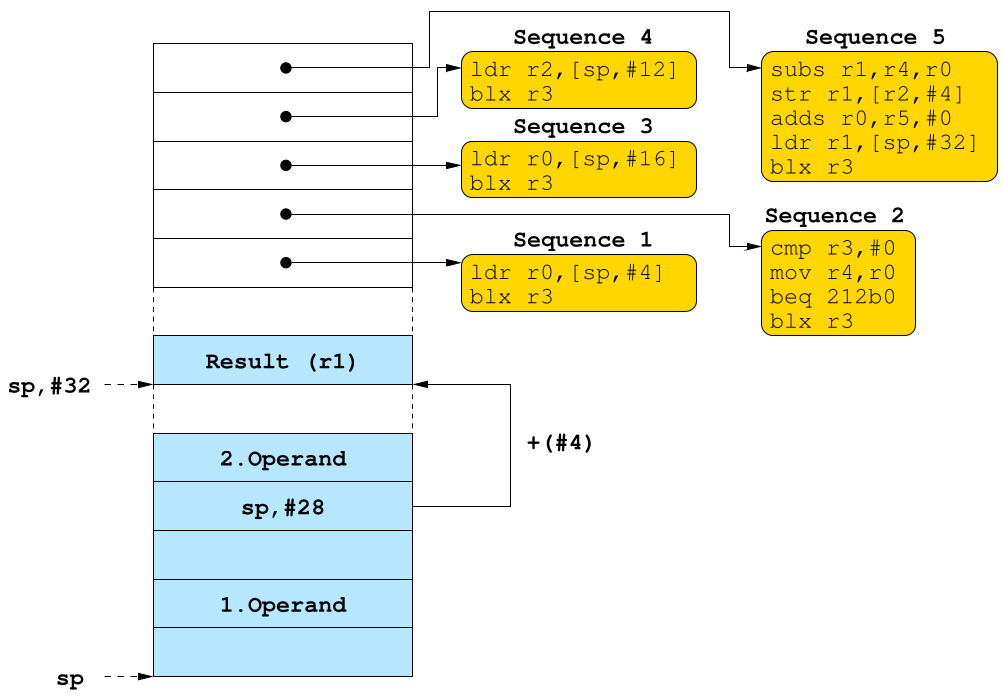
\includegraphics[scale=0.3]{gadgetARM.png}
    \end{figure}
\end{frame}

\begin{frame}
    \frametitle{Ataques Concretos: Linux Intel x86}
    
    \begin{figure}
        \centering
        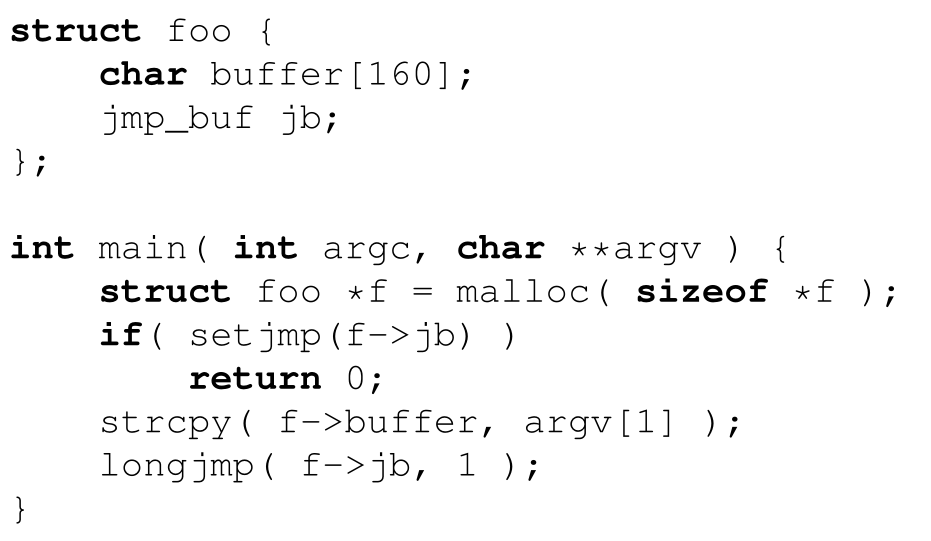
\includegraphics[width=0.9\textwidth]{LinuxIntel86.png}
    \end{figure}
        
    
\end{frame}

\begin{frame}
    \frametitle{Ataques Concretos: Google Android ARM}
    \begin{figure}
        \centering
        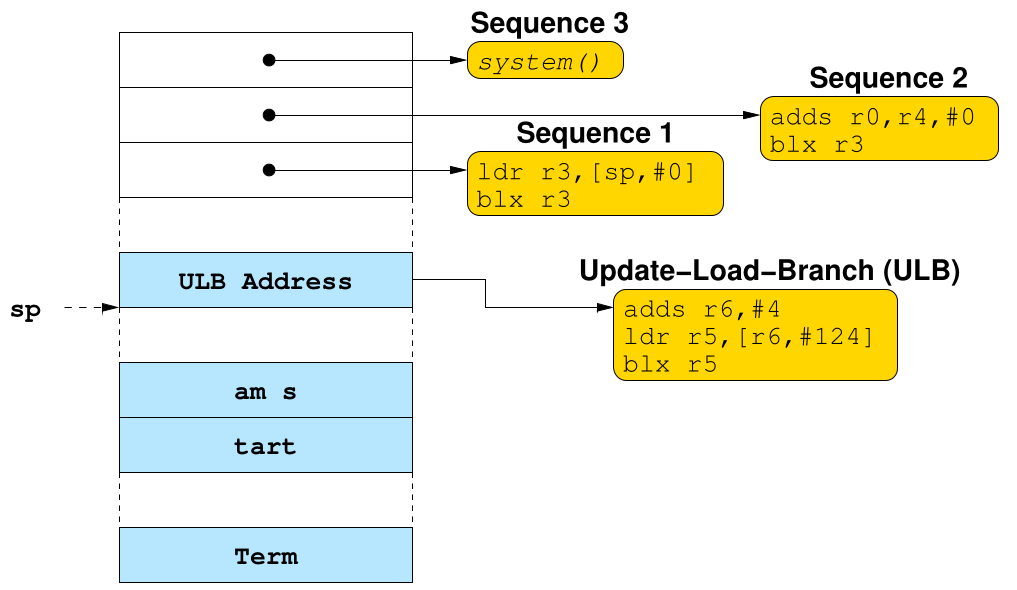
\includegraphics[width=0.8\textwidth]{GoogleAndroidARM.png}
    \end{figure}
        
    Obtener una shell en el emulador para el desarrollador de android.\\
    Se utiliza el mismo código a traves de una interfaz de java para C.
\end{frame}

\begin{frame}
    \frametitle{Conclusiones}
    \begin{itemize}
        \item Encontrar un trampolín basta para construir a su alrededor un conjunto de \textit{gadgets}.
        \item Esta nueva forma de programar es un problema grave de seguridad.
        \item Las posibles mitigaciones pueden tener una gran penalidad.
    \end{itemize}
\end{frame}


\end{document}